\section{Analysis of the results}
\newcolumntype{C}{>{\Centering\arraybackslash\hspace{0pt}}X}

\subsection{Presentation of the data}

\subsubsection{Tabular presentation}

The arithmetic mean of a decimal place was caluclated for 100 trials and the data points 
in the table shown below were found (rounded to 3 s.f.):

\begin{table}[h]
    \noindent% <-- important
    \setlength\tabcolsep{3pt} % default: 6pt
    \begin{tabularx}{\textwidth}{@{} l *{6}{C} @{}}
    \toprule
    Decimal place & Average time for approximation using Viete's method, in milliseconds (ms) & Average time for approximation using Madhava's method method, in milliseconds (ms) \\ 
    \midrule
    5  & 0.760  & 0.592   \\
    10 & 1.29  & 1.31    \\
    15 & 2.05  & 1.9     \\
    20 & 2.64  & 2.68    \\
    25 & 3.09  & 3.21    \\
    30 & 3.82  & 3.9     \\
    35 & 4.44  & 4.55    \\
    40 & 5.08  & 5.26    \\
    45 & 5.71  & 5.84    \\
    50 & 6.37  & 6.58    \\
    55 & 7.02  & 7.27    \\
    60 & 7.72  & 8.00   
    \end{tabularx}
\end{table}

\pgfplotstableread{
    X Y
    5 0.7601666451
    10 1.288158894
    15 2.050116062 
    20 2.63982296 
    25 3.091802597
    30 3.819538355 
    35 4.442822933
    40 5.081979036 
    45 5.706284046 
    50 6.370962858 
    55 7.020516396 
    60 7.723451853   
}\vietetable

\pgfplotstableread{
    X Y
    5 0.5919837952 
    10 1.307063103  
    15 1.902475357  
    20 2.679748535  
    25 3.212277889  
    30 3.904948235  
    35 4.547913074  
    40 5.255579948  
    45 5.837199688  
    50 6.578524113  
    55 7.270073891  
    60 8.004565239  

}\madhavatable

\subsubsection{Graphical presentation}

To better show the trend in the data collected, the data 
has been presented in a scatter chart below. The blue markers and line of best-fit 
respresent the results received from Viète's method while the red represent those 
from Madhava's method. 


\begin{tikzpicture}[scale=1.1]
    \begin{axis}[
        title={Comparing the time taken for approximating the value of $\pi$},
        xlabel={Decimal places},
        ylabel={Time taken [ms]},
        xmin=0, xmax=60,
        ymin=0, ymax=10,
        ytick={0,2,4,6,8,10},
        xtick={0,10,20,30,40,50,60},
        legend pos=north west,
        ymajorgrids=true,
        grid style=dashed,
        scale=1.2
    ]
    
    \addplot[
        only marks,
        color=blue,
        mark=*,
        ] table {\vietetable};
        \legend{Viète's method}
        
    \addplot [thin, blue] table[
        y={create col/linear regression={y=Y}}
    ] % compute a linear regression from the input table
    {\vietetable};
    \addlegendentry{best fit line}



    \addplot[
        only marks,
        color=red,
        mark=*,
        ] table {\madhavatable};
        \addlegendentry{Madhava's method}
        
    \addplot [thin, red] table[
        y={create col/linear regression={y=Y}}
    ] % compute a linear regression from the input table
    {\madhavatable};
    \addlegendentry{best fit line}

    \end{axis}
\end{tikzpicture}

\subsection{Observations and analysis}

The results gathered from this experiment show linear relationship between the amount of decimal 
places approximated and the time required for this approximation. The two lines of best fit for 
the two methods show similarities but also differences. It can be firstly noted that Madhava's 
method is faster than the other until the decimal 20, when the two best fit lines diverge. This 
can be explained as due to the convergence rates of the two methods, which can be seen in (Figure 3) 
\ref{fig:comparaison}. In the beginning of this curve representing the convergence of Viète's method, 
it cna be seen that it does not follow an \textit{alternating} method, like the one formulated by 
Madhava. Madhava's method is what is called an alternating series, in this case one that converges 
to the value $\pi$ \footnote{Note: not all alternating series converge}



\begin{figure}
    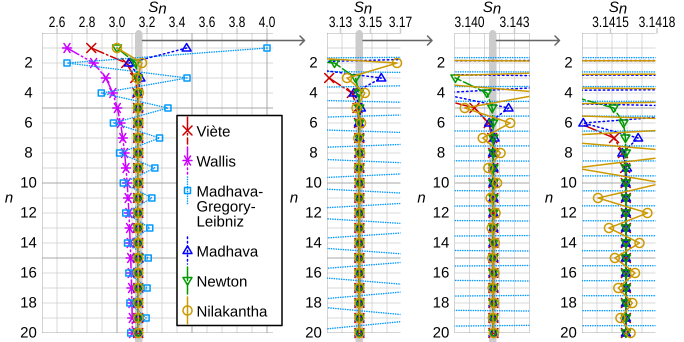
\includegraphics[width=\linewidth]{image.png}
    \caption{Comparison of historical methods of approximating the value of $\pi$. This image demonstrates
    their convergence rates. The line labelled Madhava in dark blue is the method used in this paper. 
    From (Wikimedia Commons) \cite{infinite_series_comparaison}}
    \label{fig:comparaison}
  \end{figure}
